\documentclass[11pt]{article}
% Font tiếng việt
\usepackage{fontspec}
\usepackage[vietnamese]{babel}

% Sử dụng bảng dài có thể ngắt trang
\usepackage{longtable}
\usepackage{ragged2e}

\usepackage{graphicx}
\usepackage{amsmath, amssymb, amsfonts, bm}
\usepackage{xcolor}
\usepackage{hyperref}
\usepackage{pifont}
\newcommand{\xmark}{\ding{55}}
\newcommand{\cmark}{\ding{51}}
\usepackage{array}
\usepackage{float}

\definecolor{codehighlight}{rgb}{0.95,0.95,0.92}

\hypersetup{
    colorlinks=true,
    linkcolor=blue,
    filecolor=magenta,
    urlcolor=red,
    pdftitle={Overleaf Example},
    pdfpagemode=FullScreen,
}

\setmainfont{Times New Roman}

% Page layout
\setlength{\topmargin}{-.5in}
\setlength{\textheight}{9.25in}
\setlength{\oddsidemargin}{0in}
\setlength{\textwidth}{6.8in}

\usepackage{titling}
\setlength{\droptitle}{-10em}

\renewcommand{\maketitle}{%
    \begin{center}
        \fontsize{18}{20}\selectfont\textbf{Module 3 Tuần 1 - Excel for Data Analysis phần 1}\\[1em]
        \fontsize{14}{16}\selectfont Time-Series Team\\[0.5em]
        \fontsize{14}{16}\selectfont Ngày 2 tháng 8 năm 2025
    \end{center}
    \vspace{1.5em}
}

\usepackage{titlesec}
\titleformat{\section}
{\normalfont\Large\bfseries}
{}{0em}{}

\usepackage{listings}
\definecolor{codegreen}{rgb}{0,0.6,0}
\definecolor{codegray}{rgb}{0.5,0.5,0.5}
\definecolor{codepurple}{rgb}{0.58,0,0.82}
\definecolor{backcolour}{rgb}{0.95,0.95,0.92}
\lstdefinestyle{mystyle}{
    backgroundcolor=\color{backcolour},
    commentstyle=\color{codegreen},
    keywordstyle=\color{magenta},
    numberstyle=\tiny\color{codegray},
    stringstyle=\color{codepurple},
    basicstyle=\ttfamily\footnotesize,
    breaklines=true,
    captionpos=b,
    keepspaces=true,
    numbers=left,
    numbersep=5pt,
    tabsize=2,
    showspaces=false,
    showstringspaces=false,
    showtabs=false
}
\lstset{style=mystyle}

\usepackage[many]{tcolorbox}
\definecolor{lightgreenbox}{rgb}{0.85,0.95,0.85}
\newtcolorbox{summarybox}{
    colback = lightgreenbox,
    colframe = green!50!black,
    boxsep = 5pt,
    arc = 4pt,
    outer arc = 4pt,
    boxrule = 0.5pt,
    left = 10pt,
    right = 10pt,
    top = 10pt,
    bottom = 10pt,
    fontupper = \setmainfont{Times New Roman}\normalfont,
}

\usepackage{lipsum}
\newcounter{mycounter}
\newcommand\showmycounter{\stepcounter{mycounter}\themycounter}
\newcommand\showlips{\stepcounter{mycounter}\lipsum[\value{mycounter}]}

\usepackage{booktabs}
\usepackage{subcaption}
\usepackage{framed}
\usepackage{tikz}

\begin{document}

\maketitle

\begin{summarybox}
Buổi học thứ 7 (ngày 2/8/2025) được chia thành 3 phần chính nhằm giúp ta hiểu cách sử dụng Excel cho phân tích dữ liệu cơ bản, thống kê và trực quan hóa:
\begin{itemize}
    \item \textbf{Phần 1: Hiểu Tổng Quan Về Phân Tích Dữ Liệu} – Khái niệm dữ liệu, quy trình và ứng dụng Excel.
    \item \textbf{Phần 2: Hiểu Xu Hướng Dữ Liệu Qua Thống Kê Cơ Bản} – Phương pháp thống kê và Pivot Table để phát hiện xu hướng.
    \item \textbf{Phần 3: Trực Quan Hóa Dữ Liệu} – Tạo biểu đồ, dashboard với tips hiệu quả.
\end{itemize}
\end{summarybox}
\section{Phần 1: Hiểu Tổng Quan Về Phân Tích Dữ Liệu}

\subsection{Định nghĩa Dữ liệu và Thông tin}
Dữ liệu (Data) là các sự kiện thô, chưa qua xử lý, thường ở dạng số, ký tự, hình ảnh và chưa mang nhiều ý nghĩa.
Thông tin (Information) là dữ liệu đã được xử lý và có ngữ cảnh rõ ràng, hỗ trợ ra quyết định.

\begin{itemize}
    \item \textbf{Dữ liệu:} Thô, ví dụ: \texttt{15.000.000}, \texttt{42\%}, \texttt{"TPHCM"}.
    \item \textbf{Thông tin:} Ví dụ: \texttt{"Doanh thu tháng 6 là 15 triệu đồng, tăng 42\% so với TPHCM"}.
\end{itemize}

\begin{figure}[H]
    \centering
    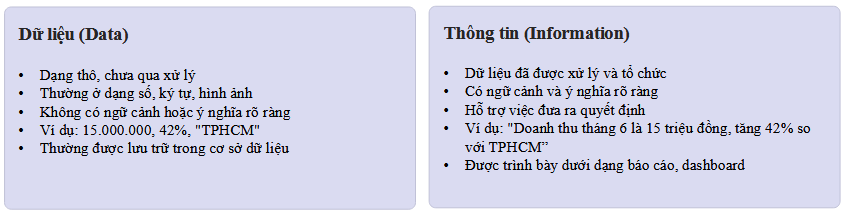
\includegraphics[width=1\linewidth]{images/data_vs_infor.png}
    \caption{Data vs Information}
    \label{fig:data_vs_info}
\end{figure}

\subsection{Sự bùng nổ dữ liệu toàn cầu}
Khối lượng dữ liệu toàn cầu đã tăng mạnh trong hơn một thập kỷ qua, từ 2 zettabyte năm 2010 lên tới hơn 180 zettabyte vào năm 2025 (dự kiến). Xu thế này cho thấy việc biết cách phân tích dữ liệu trở nên quan trọng để tìm ra giá trị từ khối lượng thông tin khổng lồ đó.

\begin{figure}[H]
    \centering
    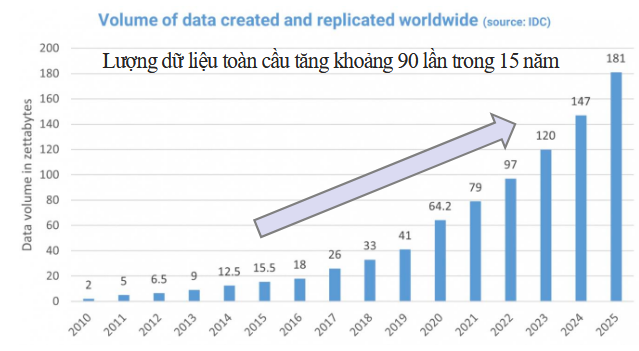
\includegraphics[width=1\linewidth]{images/dataExplosion.png}
    \caption{Data Explosion}
    \label{fig:dataExplosion}
\end{figure}

\subsection{Quy trình phân tích dữ liệu}
\begin{enumerate}
    \item \textbf{Xác định vấn đề:} Bắt đầu với câu hỏi đúng, xác định chỉ số kinh doanh cần phân tích.
    \item \textbf{Thu thập dữ liệu:} Lấy dữ liệu từ cơ sở dữ liệu, file, API, khảo sát.
    \item \textbf{Làm sạch dữ liệu:} Xử lý dữ liệu thiếu, loại bỏ trùng lặp, ngoại lai.
    \item \textbf{Khám phá dữ liệu:} Thống kê mô tả, trực quan hoá để hiểu cấu trúc.
    \item \textbf{Phân tích \& mô hình hoá:} Áp dụng thống kê, học máy để tìm mối quan hệ.
    \item \textbf{Diễn giải \& hành động:} Chuyển kết quả thành insight, hỗ trợ quyết định.
\end{enumerate}
Trong bài ngày hôm nay, chúng ta sẽ đi từ tổng quan tới từng truy trình để phân tích dữ liệu với ví dụ cụ thể (i.e. use case) và vì sao mình nên dùng Excel cho công việc có dữ liệu < 1 triệu mẫu thay vì dùng Code để phân tích mất nhiều thời gian.


\subsection{Lợi ích của phân tích dữ liệu}
Phân tích dữ liệu giúp các quyết định bớt phụ thuộc vào cảm tính. Nó cho phép phát hiện sớm xu hướng, dự báo nhu cầu để quản lý tồn kho, tối ưu quy trình để giảm lãng phí, và cá nhân hóa trải nghiệm khách hàng. Những lợi ích này đều góp phần cải thiện hiệu quả hoạt động và tăng giá trị cho tổ chức.

\subsection{Lý do nên học phân tích dữ liệu}
Kỹ năng phân tích dữ liệu mở ra nhiều cơ hội nghề nghiệp như Data Analyst, Data Scientist hay Data Engineer. Ngoài ra, khả năng tư duy phân tích được đánh giá cao trong nhiều lĩnh vực và thường được nhắc đến trong các báo cáo về xu hướng việc làm toàn cầu.

\begin{figure}[H]
    \centering
    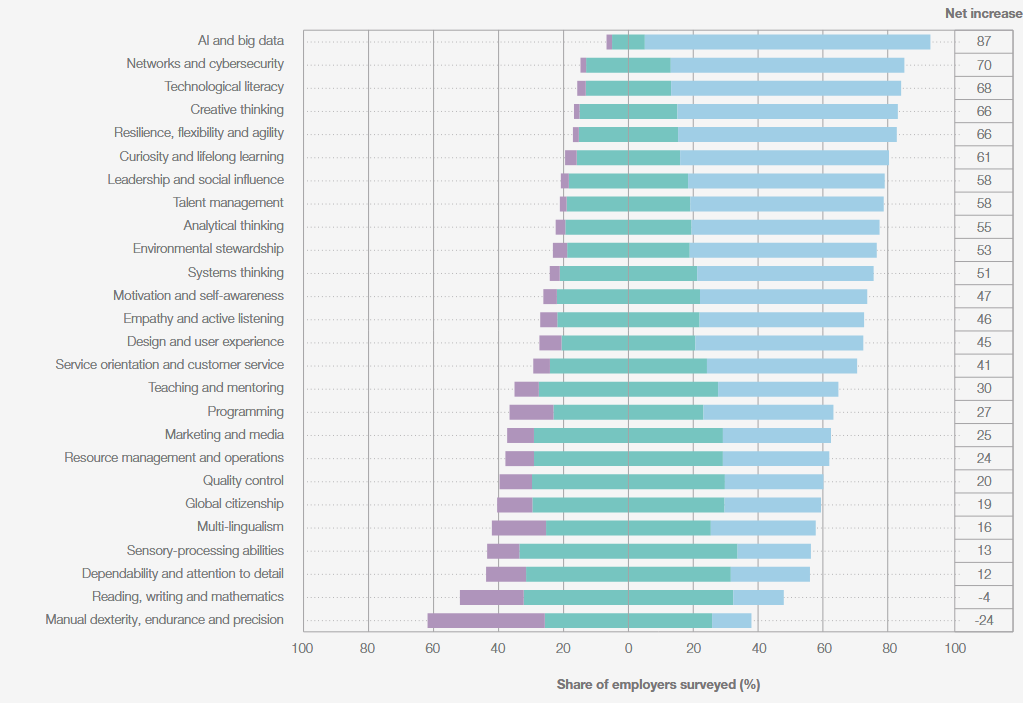
\includegraphics[width=1\linewidth]{images/whyStudyDA.png}
    \caption{Top những ngành lên trend nhiều nhất theo \%}
    \label{fig:job increase 2025 in percent}
\end{figure}

\subsection{Các vai trò phổ biến trong lĩnh vực dữ liệu}
Trong ngành này có 3 vai trò chính. Data Scientist thường tập trung vào mô hình nâng cao và học máy. Data Analyst hoặc BI Analyst chú trọng việc đặt câu hỏi kinh doanh, phân tích số liệu và xây dựng báo cáo. Data Engineer chịu trách nhiệm xây dựng hạ tầng dữ liệu và pipeline. Mỗi vai trò đều cần kỹ năng kỹ thuật kết hợp với hiểu biết về nghiệp vụ.

\begin{figure}[H]
    \centering
    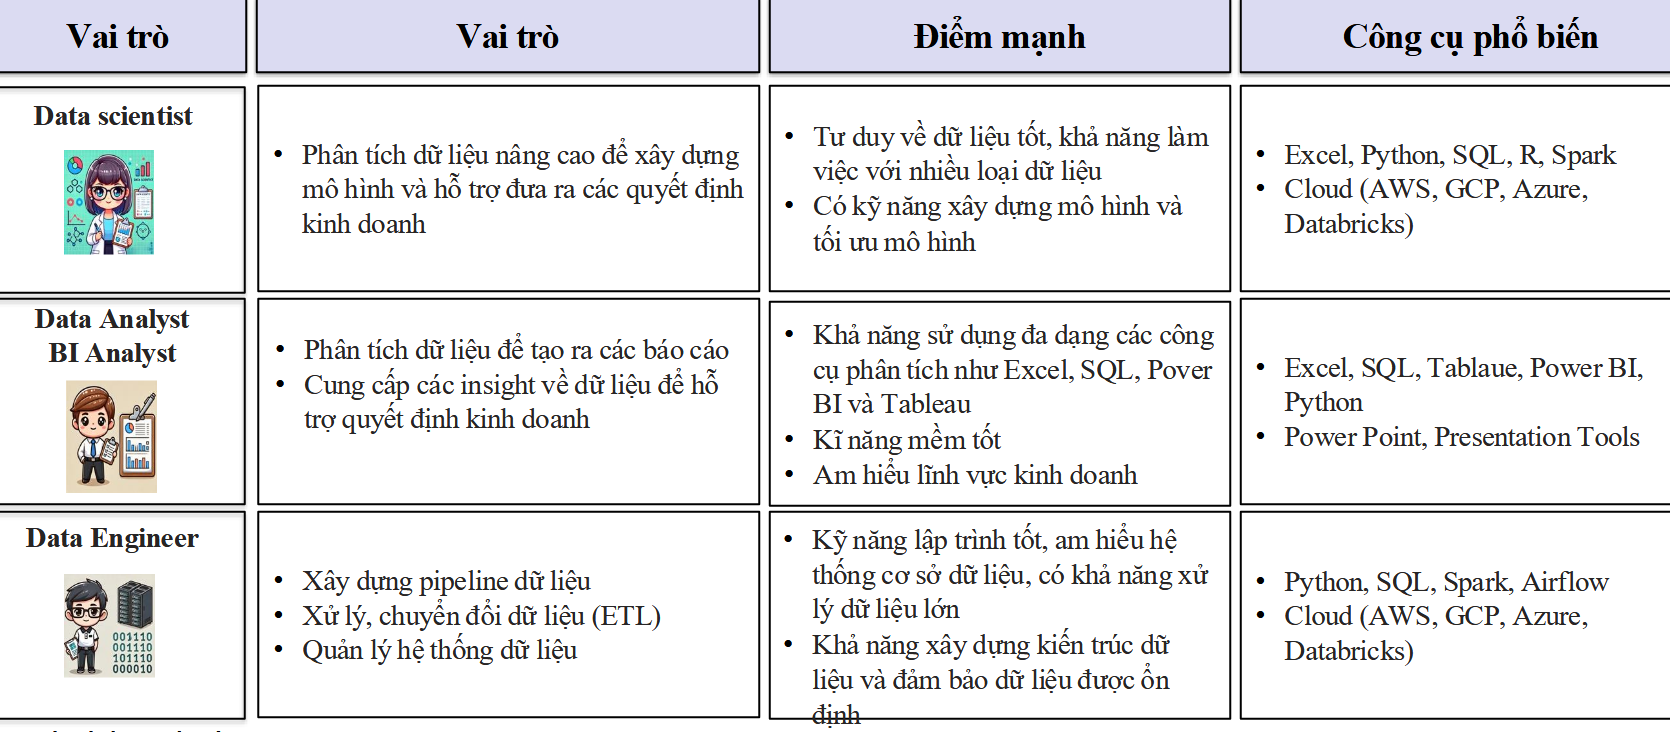
\includegraphics[width=1\linewidth]{images/jobs_in_dataAnalysis.png}
    \caption{Một số công việc liên quan đến dữ liệu}
    \label{fig:jobs_in_dataAnalysis}
\end{figure}


\subsection{Ai nên học phân tích dữ liệu}
Hầu hết mọi người đều có thể hưởng lợi từ kỹ năng này. Nhân viên văn phòng có thể tự động hóa công việc. Người làm doanh nghiệp vừa hoặc nhỏ có thể theo dõi chi phí và khách hàng. Sinh viên có thể thích ứng tốt hơn với môi trường khi biết cách tự phân tích dữ liệu, và có thể phát triển góc nhìn trực quan hơn về thị trường với kiến thức phân tích dữ liệu.

\subsection{Ứng dụng trong thực tế}
Phân tích dữ liệu được áp dụng ở nhiều lĩnh vực. Netflix và Spotify dùng để gợi ý nội dung. Trong thể thao, dữ liệu được dùng để theo dõi hiệu suất. Amazon và Walmart ứng dụng trong thương mại và quản lý chuỗi cung ứng. Trong y tế và giáo dục, phân tích dữ liệu hỗ trợ dự báo và theo dõi tiến trình.


\subsection{5 cấp độ của phân tích dữ liệu}
Có năm cấp độ thường được nhắc đến: mô tả (descriptive), quan hệ (relational), nhân quả (causal), dự báo (predictive) và tối ưu hóa (optimization). Mỗi cấp độ giúp trả lời những loại câu hỏi khác nhau, từ việc mô tả dữ liệu quá khứ đến dự đoán tương lai và tìm cách cải thiện hiệu suất.
\begin{enumerate}
    \item \textbf{Descriptive:} Hiểu quá khứ và hiện tại.
    \item \textbf{Relational:} Phát hiện mối quan hệ giữa hiện tượng.
    \item \textbf{Causal:} Tìm quan hệ nhân quả.
    \item \textbf{Predictive:} Dự đoán xu hướng tương lai.
    \item \textbf{Optimization:} Tối ưu hoá kết quả.
\end{enumerate}

\subsection{Lưu ý khi phân tích dữ liệu}
Trong phân tích dữ liệu, Ta ĐẶT BIỆT cần PHÂN BIỆT rõ giữa \textbf{SỰ THẬT} (fact) và \textbf{SUY LUẬN} (inference).
Việc phân tích nên bắt đầu từ những câu hỏi cụ thể và có mục tiêu rõ ràng. Điều này giúp tiết kiệm thời gian và tránh bị lệch hướng vì sự thật chỉ đúng khi dữ liệu theo sau.

\begin{figure}[H]
    \centering
    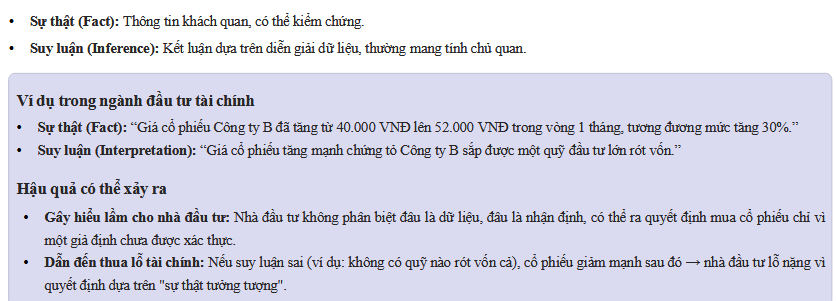
\includegraphics[width=1\linewidth]{images/fact_vs_inference.png}
    \caption{Phân biệt Fact và Inference}
    \label{fig:fact_vs_inference}
\end{figure}

\subsection{Framework 5W2H trong phân tích dữ liệu}
\section{Phần 2: Hiểu Xu Hướng Dữ Liệu Qua Thống Kê Cơ Bản}

\subsection{Tại sao cần hiểu xu hướng dữ liệu?}
Phát hiện xu hướng trong dữ liệu giúp doanh nghiệp dự báo, nhận diện bất thường và tối ưu hiệu suất. Ví dụ, hai cửa hàng điện tử có cùng doanh thu trung bình, nhưng một cửa hàng có doanh thu ổn định, cửa hàng còn lại dao động mạnh. Nếu chỉ nhìn vào giá trị trung bình, ta dễ bỏ sót sự khác biệt quan trọng này.

\begin{figure}[H]
    \centering
    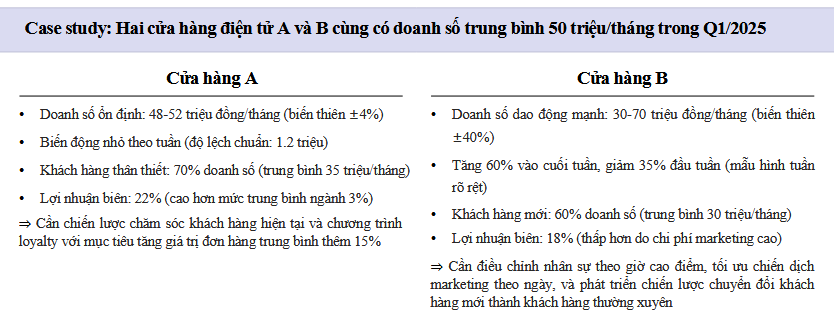
\includegraphics[width=1\linewidth]{images/caseStudy_DataTrending.png}
    \caption{Case Study: So sánh xu hướng dữ liệu}
    \label{fig:Case Study}
\end{figure}

\subsection{Không chỉ dựa vào giá trị trung bình}
Giá trị trung bình (Mean) là thước đo phổ biến để mô tả dữ liệu, nhưng có thể gây hiểu lầm nếu dữ liệu chứa ngoại lệ (outlier).
\begin{itemize}
    \item \textbf{Mean (Trung bình):} Tính bằng tổng các giá trị chia cho số lượng phần tử. Phù hợp khi dữ liệu phân bố đều và ít outlier.
	\[
        \bar{x} = \frac{1}{n} \sum_{i=1}^{n} x_i
    \]

    \item \textbf{Median (Trung vị):} Là giá trị nằm giữa khi sắp xếp dữ liệu theo thứ tự. Ít bị ảnh hưởng bởi outlier, nên nó phản ánh tốt hơn vị trí trung tâm khi dữ liệu lệch hoặc có giá trị cực đoan.
    \[
        Median =
        \begin{cases}
            x_{\frac{n+1}{2}}, & \text{n lẻ} \\[6pt]
            \frac{x_{\frac{n}{2}} + x_{\frac{n}{2}+1}}{2}, & \text{n chẵn}
        \end{cases}
    \]
\end{itemize}

\textbf{Ví dụ:} Thu nhập của 5 nhân viên lần lượt là \{10, 12, 14, 15, 100\} triệu.
\begin{itemize}
    \item Mean = (10+12+14+15+100)/5 = 30.2 triệu → bị kéo lên bởi giá trị 100 triệu.
    \item Median = 14 triệu → phản ánh mức điển hình hơn cho phần lớn nhân viên.
\end{itemize}

\begin{figure}[H]
    \centering
    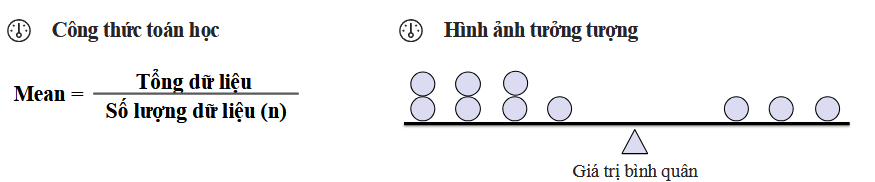
\includegraphics[width=1\linewidth]{images/mean_vs_median.png}
    \caption{So sánh Mean và Median}
    \label{fig:mean vs median}
\end{figure}


\subsection{Đo lường mức độ phân tán}
Ngoài giá trị trung tâm, cần quan tâm đến mức độ dao động của dữ liệu. Hai chỉ số thường dùng là:

\begin{itemize}
    \item \textbf{Variance (Phương sai):} Đo lường mức độ phân tán của dữ liệu quanh giá trị trung bình. Nên dùng trong bài toán hồi quy khi cần tính giá trị bình phương cho khoảng cách.

    \[
        Var(X) = \frac{1}{n} \sum_{i=1}^{n} (x_i - \bar{x})^2
    \]

    \item \textbf{Standard Deviation (Độ lệch chuẩn):} Là căn bậc hai của phương sai, có cùng đơn vị với dữ liệu gốc nên dễ hiểu hơn. Dùng khi muốn giải thích mức độ biến động cùng đơn vị với dữ liệu gốc.

    \[
        SD(X) = \sqrt{Var(X)} = \sqrt{\frac{1}{n} \sum_{i=1}^{n} (x_i - \bar{x})^2}
    \]
\end{itemize}

\textbf{Ví dụ minh họa:}
\begin{itemize}
    \item Dữ liệu doanh thu (triệu VND): 50, 52, 49, 51, 48.
    \item Trung bình = 50.
    \item Phương sai = 2.5 (thấp) → Doanh thu dao động ít quanh 50.
    \item Độ lệch chuẩn = $\sqrt{2.5} \approx 1.58$ → Khoảng 68\% doanh thu nằm trong khoảng [48.42, 51.58].
\end{itemize}

\textbf{So sánh hai nhóm sản phẩm:}
\begin{itemize}
    \item Nhóm A: \{100, 105, 95, 102, 98\} → Độ lệch chuẩn = 3.8 (dao động nhỏ).
    \item Nhóm B: \{80, 120, 60, 140, 100\} → Độ lệch chuẩn = 31.6 (dao động rất lớn).
    \item Cả hai nhóm đều có trung bình 100, nhưng Nhóm B rủi ro cao hơn vì biến động mạnh.
\end{itemize}

\textbf{Case study:} so sánh 2 nhóm sản phẩm sử dụng Variance và Standard Deviation trong phân tích dữ liệu.
\begin{figure}[H]
    \centering
    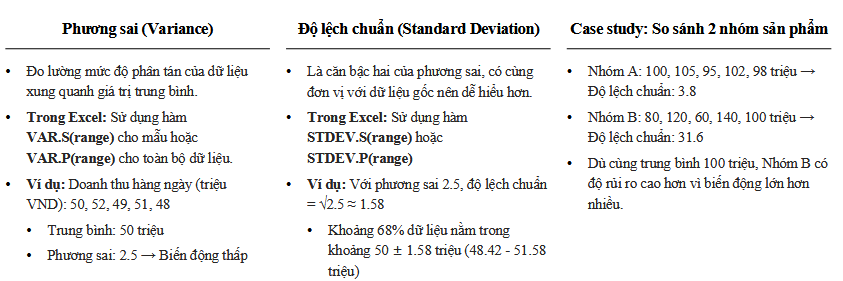
\includegraphics[width=1\linewidth]{images/variance_std_usecase.png}
    \caption{Ứng dụng Variance và Standard Deviation trong phân tích dữ liệu}
    \label{fig:variance vs std}
\end{figure}

\subsection{Một số hàm thống kê cơ bản trong Excel}
Excel cung cấp nhiều hàm thống kê hỗ trợ phân tích:
\begin{itemize}
    \item \texttt{AVERAGE()} – Tính trung bình.
    \item \texttt{MEDIAN()} – Tính trung vị.
    \item \texttt{MODE()} – Giá trị xuất hiện nhiều nhất.
    \item \texttt{VAR.P()} – Phương sai toàn bộ.
    \item \texttt{STDEV.P()} – Độ lệch chuẩn toàn bộ.
    \item \texttt{SKEW()} – Độ lệch của phân phối.
    \item \texttt{KURT()} – Độ nhọn của phân phối.
\end{itemize}

\begin{figure}[H]
    \centering
    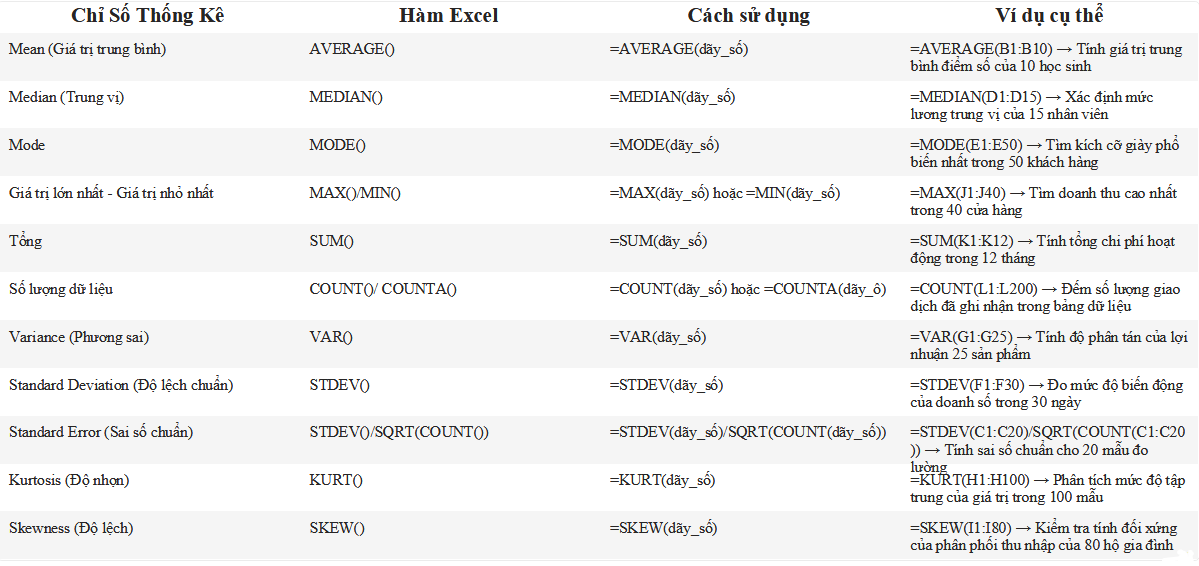
\includegraphics[width=1\linewidth]{images/stastical_func.png}
    \caption{Các hàm thống kê trong Excel}
    \label{fig:Excel Statistical FUnc}
\end{figure}

\subsection{Hàm điều kiện và tổng hợp}
Ngoài thống kê cơ bản, Excel còn hỗ trợ các hàm điều kiện giúp lọc và tính toán theo tiêu chí cụ thể:
\begin{itemize}
    \item \texttt{IF()}, \texttt{IFS()} – Hàm điều kiện.
    \item \texttt{SUMIF()}, \texttt{SUMIFS()} – Tổng có điều kiện.
    \item \texttt{COUNTIF()}, \texttt{COUNTIFS()} – Đếm có điều kiện.
    \item \texttt{AVERAGEIF()}, \texttt{AVERAGEIFS()} – Trung bình có điều kiện.
\end{itemize}

\begin{figure}[H]
    \centering
    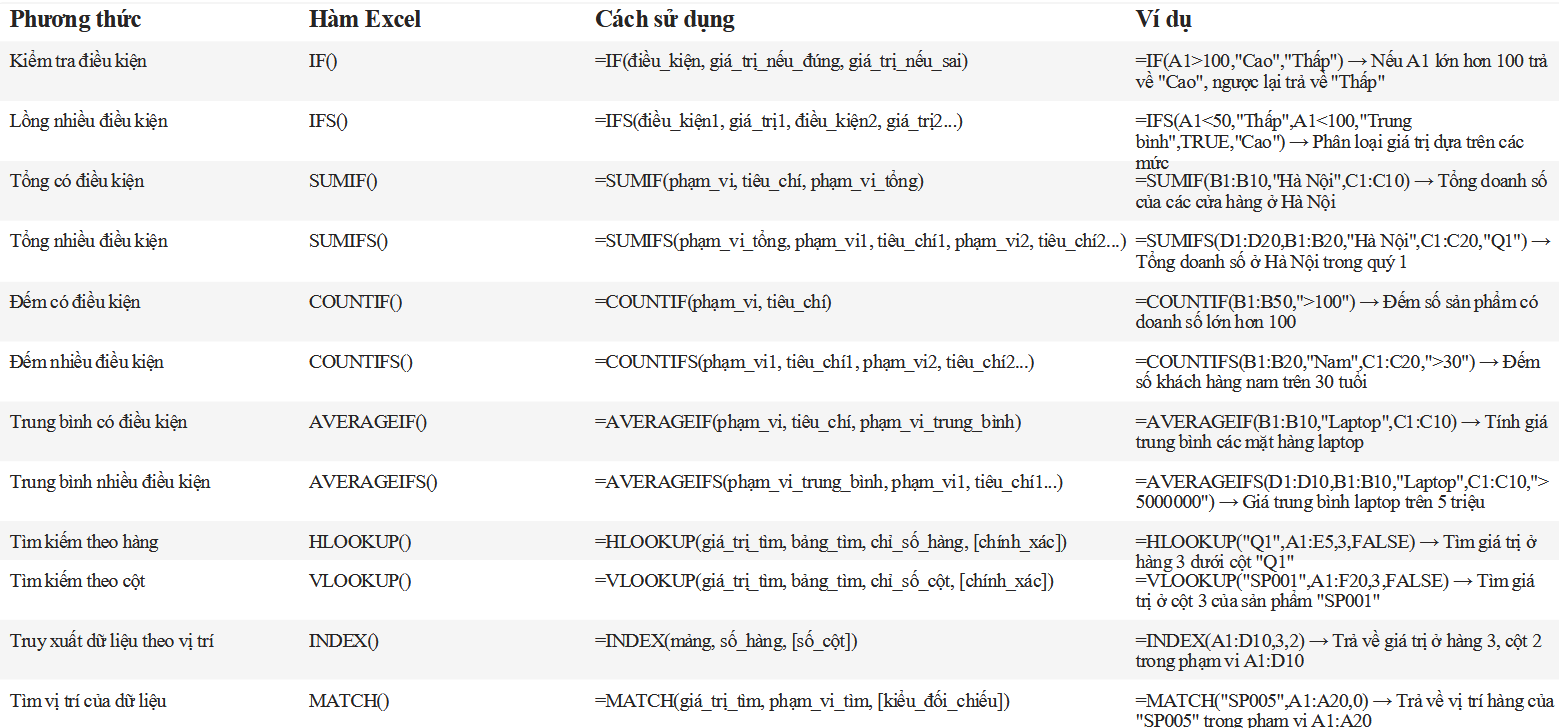
\includegraphics[width=1.2\linewidth]{images/excel_aggregation_function.png}
    \caption{Hàm tổng hợp và điều kiện trong Excel}
    \label{fig:Excel Aggregation func}
\end{figure}


\subsection{Pivot Table}
Pivot Table là công cụ mạnh trong Excel để tóm tắt dữ liệu theo nhiều chiều. Người dùng có thể kéo thả trường dữ liệu vào các ô \texttt{Rows}, \texttt{Columns}, \texttt{Values} và \texttt{Filters} để nhanh chóng tạo báo cáo động. Đây là cách đơn giản nhưng hiệu quả để phân tích tập dữ liệu lớn.

\begin{figure}[H]
    \centering
    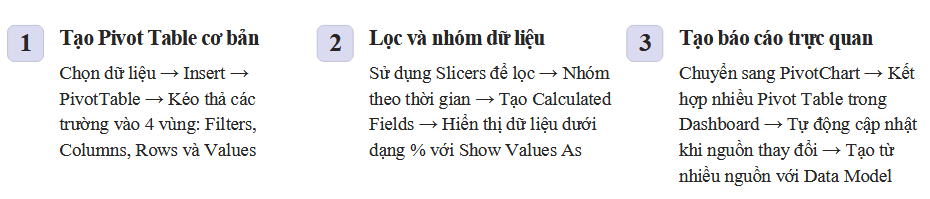
\includegraphics[width=1\linewidth]{images/pivotTable_flow.png}
    \caption{Quy trình sử dụng Pivot Table}
    \label{fig:how 2 use pivot table}
\end{figure}

\begin{figure}[H]
    \centering
    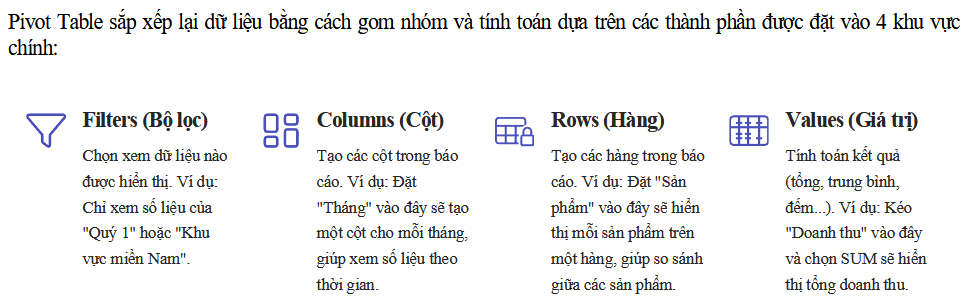
\includegraphics[width=1\linewidth]{images/pivotTable_Explain.png}
    \caption{Nguyên lý hoạt động của Pivot Table}
    \label{fig:pivot table mechanism}
\end{figure}

\section{Phần 3: Trực Quan Hóa Dữ Liệu}

\subsection{Vì sao cần trực quan hóa dữ liệu?}
Trực quan hóa giúp con người dễ dàng nhận ra xu hướng và thông tin quan trọng từ dữ liệu thô. Thay vì đọc hàng trăm dòng số liệu, biểu đồ hoặc sơ đồ cho phép nắm bắt thông điệp chỉ trong vài giây. Đây là yếu tố quan trọng trong báo cáo, thuyết trình, và hỗ trợ ra quyết định dựa trên dữ liệu. Ví dụ, minh họa dữ liệu có tính biến động theo thời gian sẽ dễ hiểu hơn thay vì dùng bản với số đơn thuần.

\begin{figure}[H]
    \centering
    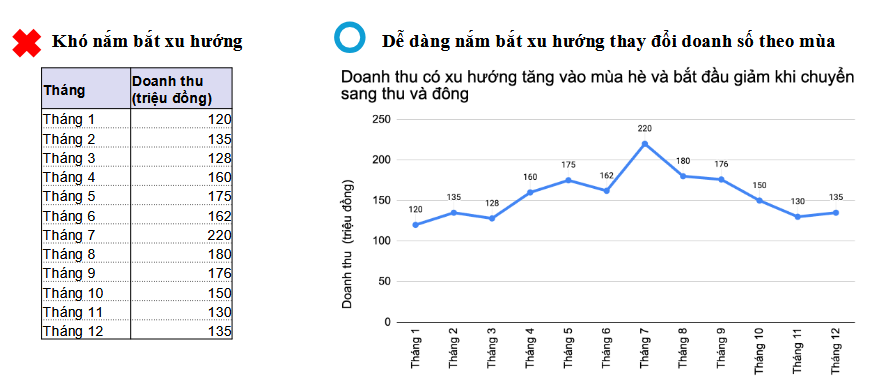
\includegraphics[width=0.7\linewidth]{images/why_dataVisualization.png}
    \caption{Tầm quan trọng của trực quan hóa dữ liệu}
    \label{fig:why DA}
\end{figure}

\subsection{Cách sử dụng biểu đồ Hiệu quả}
Một biểu đồ tốt không chỉ chính xác về mặt dữ liệu mà còn cần dễ hiểu và truyền tải thông điệp rõ ràng. Khi thiết kế biểu đồ, nên chú ý:
\begin{itemize}
    \item \textbf{Chọn đúng loại biểu đồ:} Bar chart phù hợp để so sánh, line chart để thể hiện xu hướng, pie chart để hiển thị tỷ trọng.
    \item \textbf{Đơn giản và rõ ràng:} Tránh quá nhiều màu sắc, ký hiệu hoặc chi tiết dư thừa làm rối mắt người xem.
    \item \textbf{Sử dụng nhãn và tiêu đề rõ ràng:} Đặt tên trục, đơn vị đo, chú thích (legend) nếu cần.
    \item \textbf{Nhấn mạnh thông tin chính:} Dùng màu tương phản hoặc chú thích để làm nổi bật dữ liệu quan trọng.
    \item \textbf{Tránh lạm dụng 3D hoặc hiệu ứng:} Các yếu tố này có thể làm méo mó nhận thức về dữ liệu.
\end{itemize}

\begin{figure}[H]
    \centering
    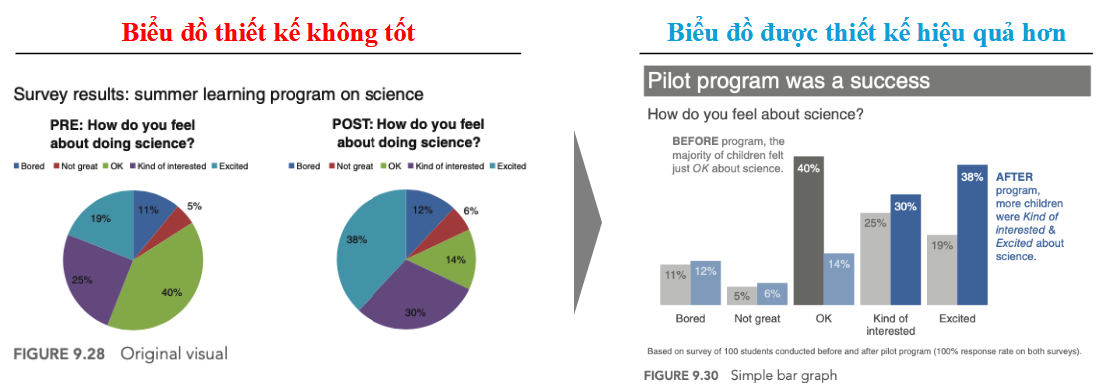
\includegraphics[width=1\linewidth]{images/bad_and_good_charttype.png}
    \caption{So sánh biểu đồ trực quan kém và hiệu quả}
    \label{fig:good vs bad chart}
\end{figure}


\subsection{Các loại biểu đồ phổ biến}
Có nhiều loại biểu đồ và sơ đồ, mỗi loại phù hợp cho một mục đích khác nhau: so sánh, theo dõi xu hướng, phân tích mối quan hệ, hoặc mô tả phân phối dữ liệu.

\begin{figure}[H]
    \centering
    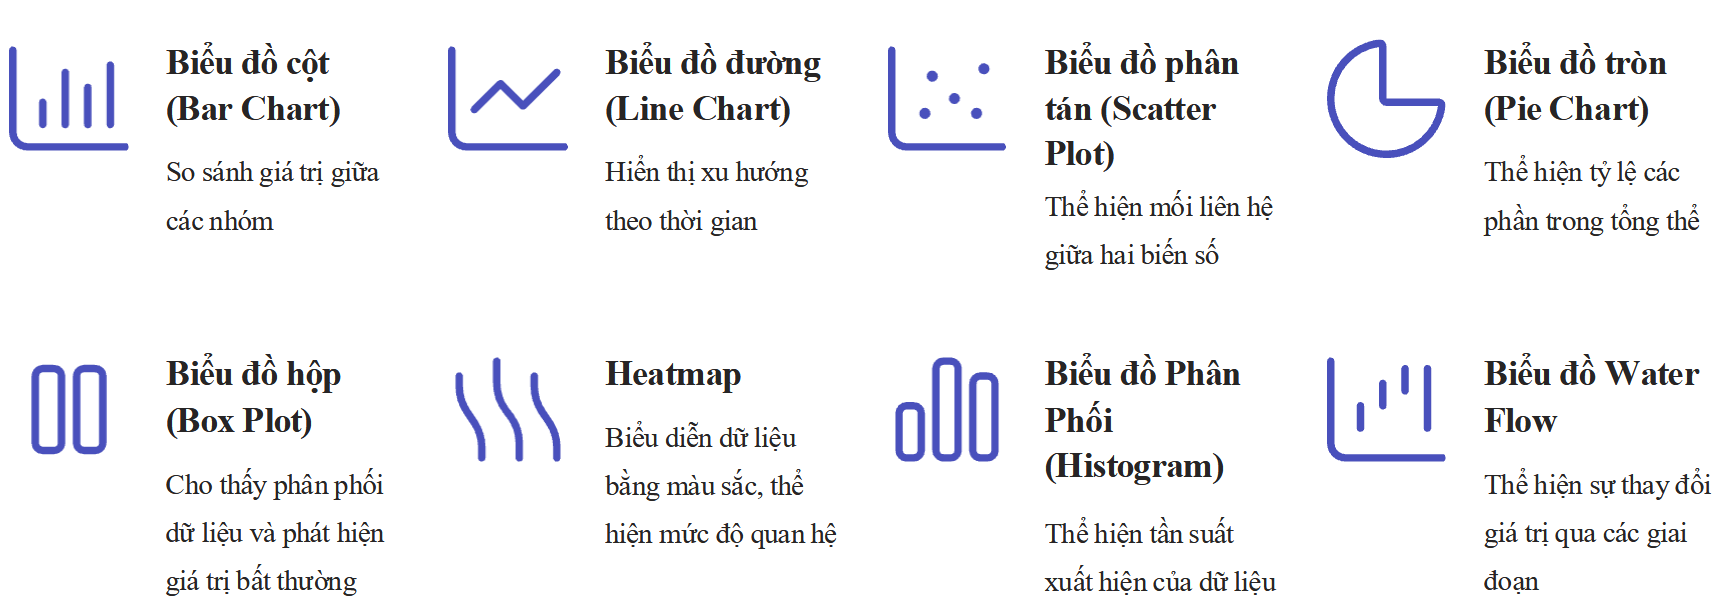
\includegraphics[width=1\linewidth]{images/visualization_chartTypes.png}
    \caption{Các loại biểu đồ, plot và diagram}
    \label{fig:chart, diagram and plot type}
\end{figure}

\subsection{Biểu đồ cột (Bar Chart)}
Dùng để so sánh giá trị giữa các nhóm hoặc hạng mục.
\textbf{Ví dụ:} So sánh doanh số bán hàng của các chi nhánh trong cùng một tháng.

\begin{figure}[H]
    \centering
    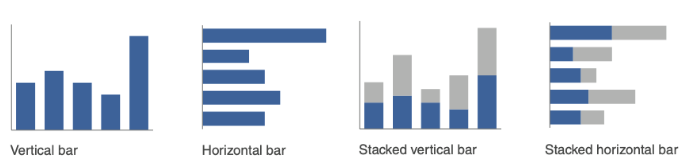
\includegraphics[width=0.9\linewidth]{images/barPlot.png}
    \caption{Ví dụ về Bar Chart}
    \label{fig:bar plot}
\end{figure}

\subsection{Biểu đồ đường (Line Chart)}
Phù hợp để thể hiện xu hướng theo thời gian.
\textbf{Ví dụ:} Theo dõi doanh thu hàng tháng trong một năm, hoặc lượng truy cập website theo ngày.

\begin{figure}[H]
    \centering
    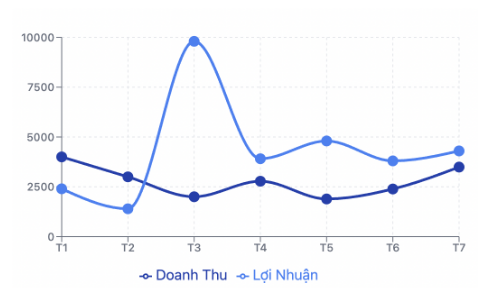
\includegraphics[width=0.6\linewidth]{images/lineChart.png}
    \caption{Ví dụ về Line Chart}
    \label{fig:line chart}
\end{figure}

\subsection{Biểu đồ tròn (Pie Chart)}
Hiển thị tỷ trọng các thành phần trong tổng thể. Chỉ nên dùng khi số nhóm ít (dưới 7).
\textbf{Ví dụ:} Tỷ lệ khách hàng theo khu vực (Bắc, Trung, Nam), hoặc Tỷ lệ bán của Máy tính bàn, điện thoại, máy tính bảng và các sản phẩm khác.

\begin{figure}[H]
    \centering
    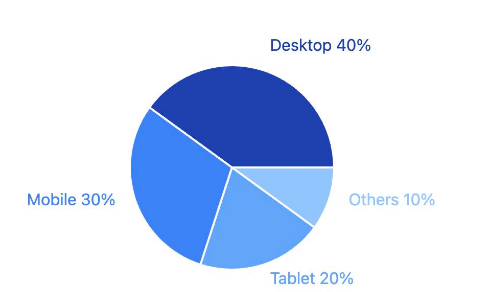
\includegraphics[width=0.6\linewidth]{images/pieChart.png}
    \caption{Ví dụ về Pie Chart}
    \label{fig:piechart}
\end{figure}

\subsection{Histogram}
Dùng để mô tả phân phối dữ liệu và tần suất xuất hiện.
\textbf{Ví dụ:} Phân phối điểm thi của sinh viên, hoặc độ tuổi khách hàng trong một cửa hàng.

\begin{figure}[H]
    \centering
    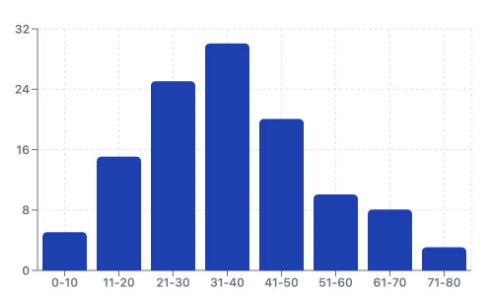
\includegraphics[width=0.6\linewidth]{images/histogram.png}
    \caption{Ví dụ về Histogram}
    \label{fig:histogram}
\end{figure}

\subsection{Heatmap}
Dùng màu sắc để biểu diễn cường độ hoặc giá trị, dễ nhận biết vùng mạnh – yếu.
\textbf{Ví dụ:} Ma trận tương quan giữa các doanh thu và lợi nhuận theo từng tháng.

\begin{figure}[H]
    \centering
    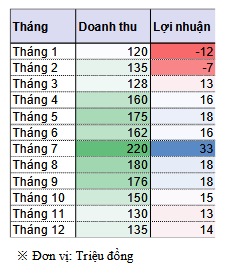
\includegraphics[width=0.6\linewidth]{images/heatmap.png}
    \caption{Ví dụ về Heatmap}
    \label{fig:heatmap}
\end{figure}

\subsection{Waterfall Chart}
Minh họa sự thay đổi tích lũy của một chỉ số qua các yếu tố cộng/trừ.
\textbf{Ví dụ:} Phân tích lợi nhuận ròng từ doanh thu, trừ chi phí và thuế để ra kết quả cuối cùng.

\begin{figure}[H]
    \centering
    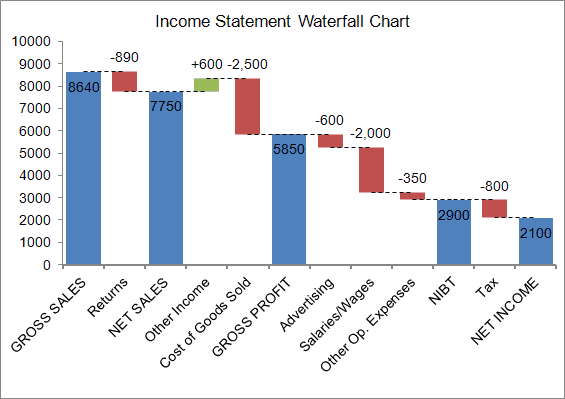
\includegraphics[width=0.7\linewidth]{images/waterFlow.png}
    \caption{Ví dụ về Waterfall Chart}
    \label{fig:waterFlow}
\end{figure}

\begin{figure}[H]
    \centering
    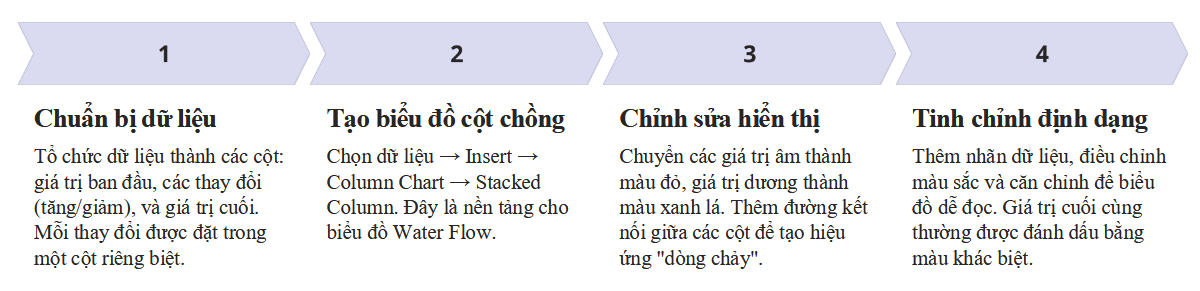
\includegraphics[width=0.7\linewidth]{images/howTo_WaterFlow.png}
    \caption{Nguyên lý xây dựng Waterfall Chart}
    \label{fig:How 2 waterFlow}
\end{figure}

\subsection{Scatter Plot}
Dùng để xem mối quan hệ giữa hai biến. Có thể thêm đường hồi quy để đánh giá xu hướng.
\textbf{Ví dụ:} So sánh số giờ học và điểm thi của sinh viên, hoặc mức chi tiêu quảng cáo và doanh số bán hàng.

\begin{figure}[H]
    \centering
    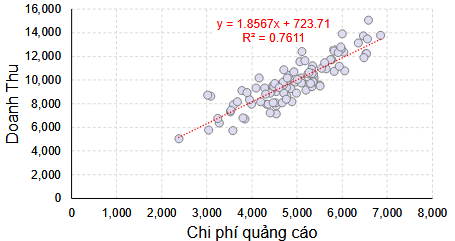
\includegraphics[width=1\linewidth]{images/scatterPlot_4_CorrelationAnalysis.png}
    \caption{Ví dụ về Scatter Plot}
    \label{fig:chart_types}
\end{figure}

\subsection{Hệ số tương quan (Correlation Coefficient)}

Hệ số tương quan cho ta biết mức độ và chiều hướng mối quan hệ tuyến tính giữa hai biến số. Giá trị này nằm trong khoảng từ -1 đến +1:

\begin{figure}[H]
    \centering
    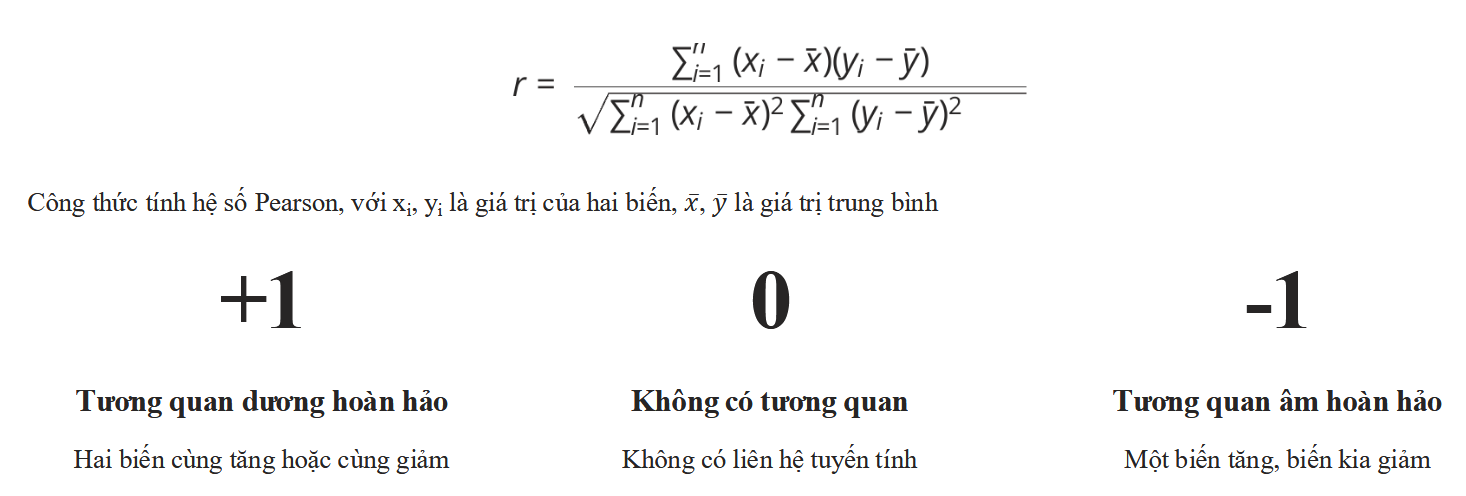
\includegraphics[width=0.7\linewidth]{images/pearson.png}
    \caption{Hệ số tương quan}
    \label{fig:pearson}
\end{figure}


\begin{itemize}
    \item Gần +1: Hai biến có mối quan hệ tuyến tính \textbf{cùng chiều mạnh} (biến A tăng thì biến B cũng tăng).
    \item Gần -1: Hai biến có mối quan hệ tuyến tính \textbf{ngược chiều mạnh} (biến A tăng thì biến B giảm).
    \item Gần 0: Không tồn tại mối quan hệ tuyến tính rõ ràng.
\end{itemize}

\textbf{Cách phân tích:}
\begin{itemize}
    \item Giá trị lớn về độ lớn (|r| gần 1) → Mối quan hệ đáng tin cậy hơn, có thể dự đoán biến này dựa trên biến kia.
    \item Giá trị nhỏ (|r| gần 0) → Quan hệ yếu, cần kiểm tra thêm hoặc dùng mô hình phi tuyến.
    \item Lưu ý: Tương quan không có nghĩa là quan hệ nhân quả. Ví dụ: số kem bán ra và số vụ đuối nước cùng tăng vào mùa hè, nhưng không phải nguyên nhân trực tiếp.
\end{itemize}

\textbf{Khi nào dùng CORREL hoặc PEARSON trong Excel:}
\begin{itemize}
    \item \texttt{=CORREL(array1, array2)}: Hàm ngắn gọn, trực tiếp trả về hệ số tương quan Pearson. Dùng khi chỉ cần kiểm tra nhanh mối liên hệ giữa hai biến.
    \item \texttt{=PEARSON(array1, array2)}: Cho cùng kết quả như CORREL, nhưng rõ ràng về mặt ý nghĩa thống kê. Nên dùng khi làm báo cáo hoặc tài liệu học thuật để nhấn mạnh đây là hệ số Pearson.
\end{itemize}



\end{document}